\subsection{Additionnal background}

The purpose of this appendix is to provide additionnal definitions and properties regarding Lipschitz Neural Networks, their possible GNP properties and Differential Privacy.

    \subsubsection{Lipschitz neural networks background}\label{sec:lipdefs}
    
    For simplicity of the exposure, we will focus on feedforward neural networks with densely connected layers: the affine transformation takes the form of a matrix-vector product $h\mapsto Wh$. In Section~\ref{sec:convnet} we tackle the case of convolutions $h\mapsto\Psi*h$ with kernel $\Psi$.  

    \begin{definition}[Feedforward neural network]\label{def:feedforward} 
        A feedforward neural network of depth $T$, with input space $\X\subset\Reals^n$, and with parameter space $\Theta\subset \Reals^p$, is a parameterized function $f:\Theta\times\X\rightarrow\Y$ defined by the following recursion:
        \begin{align}
            h_0(x) &\defeq x,\quad &
            z_t(x) &\defeq W_th_{t-1}(x)+b_t,\nonumber \\
            h_t(x) &\defeq \sigma(z_t(x)),\quad &
            f(\theta,x) &\defeq z_{T+1}(x).
        \end{align}
        The set of parameters is denoted as $\theta=(W_t,b_t)_{1\leq t\leq T+1}$, the output space as $\Y\subset\Reals^K$ (e.g logits), and the \textit{layer-wise} activation as $\sigma:\Reals^n\rightarrow\Reals^n$. 
    \end{definition}

    \begin{definition}[Lipschitz constant]\label{def:lipconstant}
        The function $f:\Reals^m\rightarrow\Reals^n$ is said $l$-Lipschitz for $l_2$ norm if for every $x,y\in\Reals^m$ we have:
            \begin{equation}
                \|f(x)-f(y)\|_2 \leq l\|x-y\|_2.% \quad \forall x, y \in \Reals^m\times\Reals^m
            \end{equation}
        Per Rademacher's theorem~\cite{simon1983lectures}, its gradient is bounded: $\|\nabla f\|\leq l$. Reciprocally, continuous functions gradient bounded by $l$ are $l$-Lipschitz.  
    \end{definition}

    \begin{definition}[Lipschitz neural network]\label{def:lipnet}
        A Lipschitz neural network is a feedforward neural network with the additional constraints:
        \begin{itemize}
            \item the activation function $\sigma$ is $S$-Lipschitz. This is a standard assumption, frequently fulfilled in practice.
            \item the affine functions $x\mapsto Wx+b$ are $U$-Lipschitz, i.e $\|W\|_2\leq U$. This is achieved in practice with spectrally normalized matrices~\cite{yoshida2017spectral}~\cite{bartlett2017spectrally}. The feasible set is the ball $\{\|W\|_2\leq U\}$ of radius $U$ (which is convex), or a subset of thereof (not necessarily convex).  
        \end{itemize}
        As a result, the function $x\mapsto f(\theta,x)$ is $U(US)^T$-Lipschitz for all $\theta\in\Theta$. 
    \end{definition}
    
    Two strategies are available to enforce Lipschitzness:
    \begin{enumerate}
        \item With a differentiable reparametrization $\Pi:\Reals^p\rightarrow\Theta$ where $\tilde\theta=\Pi(\theta)$: the weights $\tilde\theta$ are used during the forward pass, but the gradients are back-propagated to $\theta$ through $\Pi$. This turns the training into an unconstrained optimization problem on the landscape of $\Loss\circ f\circ \Pi$.\label{enum:appreparam}
        \item With a suitable projection operator $\Pi:\Reals^p\rightarrow\Theta$: this is the celebrated Projected Gradient Descent (PGD) algorithm~\cite{bubeck2015convex} applied on the landscape of $\Loss\circ f$.\label{enum:apppgd}  
    \end{enumerate}
    For arbitrary re-parametrizations, option~\ref{enum:appreparam} can cause some difficulties: the Lipschiz constant of $\Pi$ is generally unknown. However, if $\Theta$ is convex then $\Pi$ is 1-Lipschitz (with respect to the norm chosen for the projection). To the contrary, option~\ref{enum:apppgd} elicits a broader set of feasible sets $\Theta$. For simplicity, option~\ref{enum:apppgd} will be the focus of our work.  

    \subsubsection{Gradient Norm Preserving networks}

    \begin{definition}[Gradient Norm Preserving Networks]\label{def:gnp}
        GNP networks are 1-Lipschitz neural networks with the additional constraint that the Jacobian of layers consists of orthogonal matrices:
            \begin{equation}
                \left(\Jac{f_d}{x_d}\right)^T\left(\Jac{f_d}{x_d}\right)=I.%\I. ^\tr
            \end{equation}
        This is achieved with GroupSort activation~\cite{anil2019sorting,tanielian2021approximating}, Householder activation~\cite{mhammedi2017efficient}, and orthogonal weight matrices~\cite{li2019preventing,li2019orthogonal} or orthogonal convolutions (see~\cite{achour2022existence,singla2022improved,xu2022lot} and references therein). Without biases these networks are also norm preserving: $\|f(\theta,x)\|=\|x\|.$  
    \end{definition}

    The set of orthogonal matrices (and its generalization the Stiefel manifold~\cite{absil2008optimization}) is not convex, and not even connected. Hence projected gradient approaches are mandatory: for re-parametrization methods the Jacobian $\Jac{\Pi}{\theta}$ may be unbounded which could have uncontrollable consequences on sensitivity.

    \subsubsection{Background on Differential Privacy}\label{app:dpdefs}

    \begin{definition}[Neighboring datasets]\label{def:neighbouring}
        A labelled dataset $\Dataset$ is a finite collection of input/label pairs $\Dataset=\{(x_1,y_1),(x_2,y_2),\ldots... (x_N,y_N)\}$. Two datasets $\Dataset$ and $\Dataset'$ are said to be neighbouring if they differ by at most one sample: $\Dataset'=\Dataset\cup \{(x',y')\}-\{(x_i,y_i)\}$.
    \end{definition}

    The sensitivity is also referred as algorithmic stability~\cite{bousquet2002stability}, or~bounded differences property in other fields~\cite{mcdiarmid1989method}. We detail below the building of a Gaussian mechanism from an arbitrary query of known sensitivity.

    \begin{definition}[Gaussian Mechanism]\label{def:gaussianmechanism}
        Let $f:\Dataset\rightarrow\Reals^p$ be a query accessing the dataset of known $l_2$-sensitivity $\sntv(f)$, a Gaussian mechanism adds noise sampled from $\Gaussian(0,\sigma.\sntv(f))$ to the query $f$.
    \end{definition}
    
    \begin{property}[DP of Gaussian Mechanisms]\label{prop:gaussianmechanismdp}
        Let $\mathcal{G}(f).$ be a Gaussian mechanism of $l_2$-sensitivity $S_2(f)$ adding the noise $\Gaussian(0,\sigma.S_2(f))$ to the query $f$. The DP guarantees of the mechanism are given by the following continuum: 
        $\sigma = \sqrt{2.\log(1.25/\delta)} / \epsilon.$
    \end{property}

    SGD is a composition of queries. Each of those query consists of sampling a minibatch from the dataset, and computing the gradient of the loss on the minibatch. The sensitivity of the query is proportional to the maximum gradient norm $l$, and inversely proportional to the batch size $b$. By pertubing the gradient with a Gaussian noise of variance $\sigma^2\frac{l^2}{b^2}$ the query is transformed into a Gaussian mechanism. By composing the Gaussian mechanisms we obtain the DPSGD variant, that enjoy \DP guarantees.   

    \begin{proposition}[DP guarantees for SGD, adapted from~\cite{abadi2016deep}.]\label{thm:dplipschitz}
    Assume that the loss fulfills $\|\nabla_{\theta}\Loss(\yhat,y)\|_2\leq l$, and assume that the network is trained on a dataset of size $N$ with SGD algorithm for $T$ steps with noise scale $\mathcal{N}(\bf 0, \sigma^2)$ such that:
    \begin{equation}
        \sigma\geq \frac{16K\sqrt{T\log{(2/\delta)}\log{(1.25T/\delta N)}}}{N\epsilon}.
    \end{equation}
    Then the SGD training of the network is $(\epsilon,\delta)$-DP.
    \end{proposition}


    \begin{figure}[t]
        \centering
        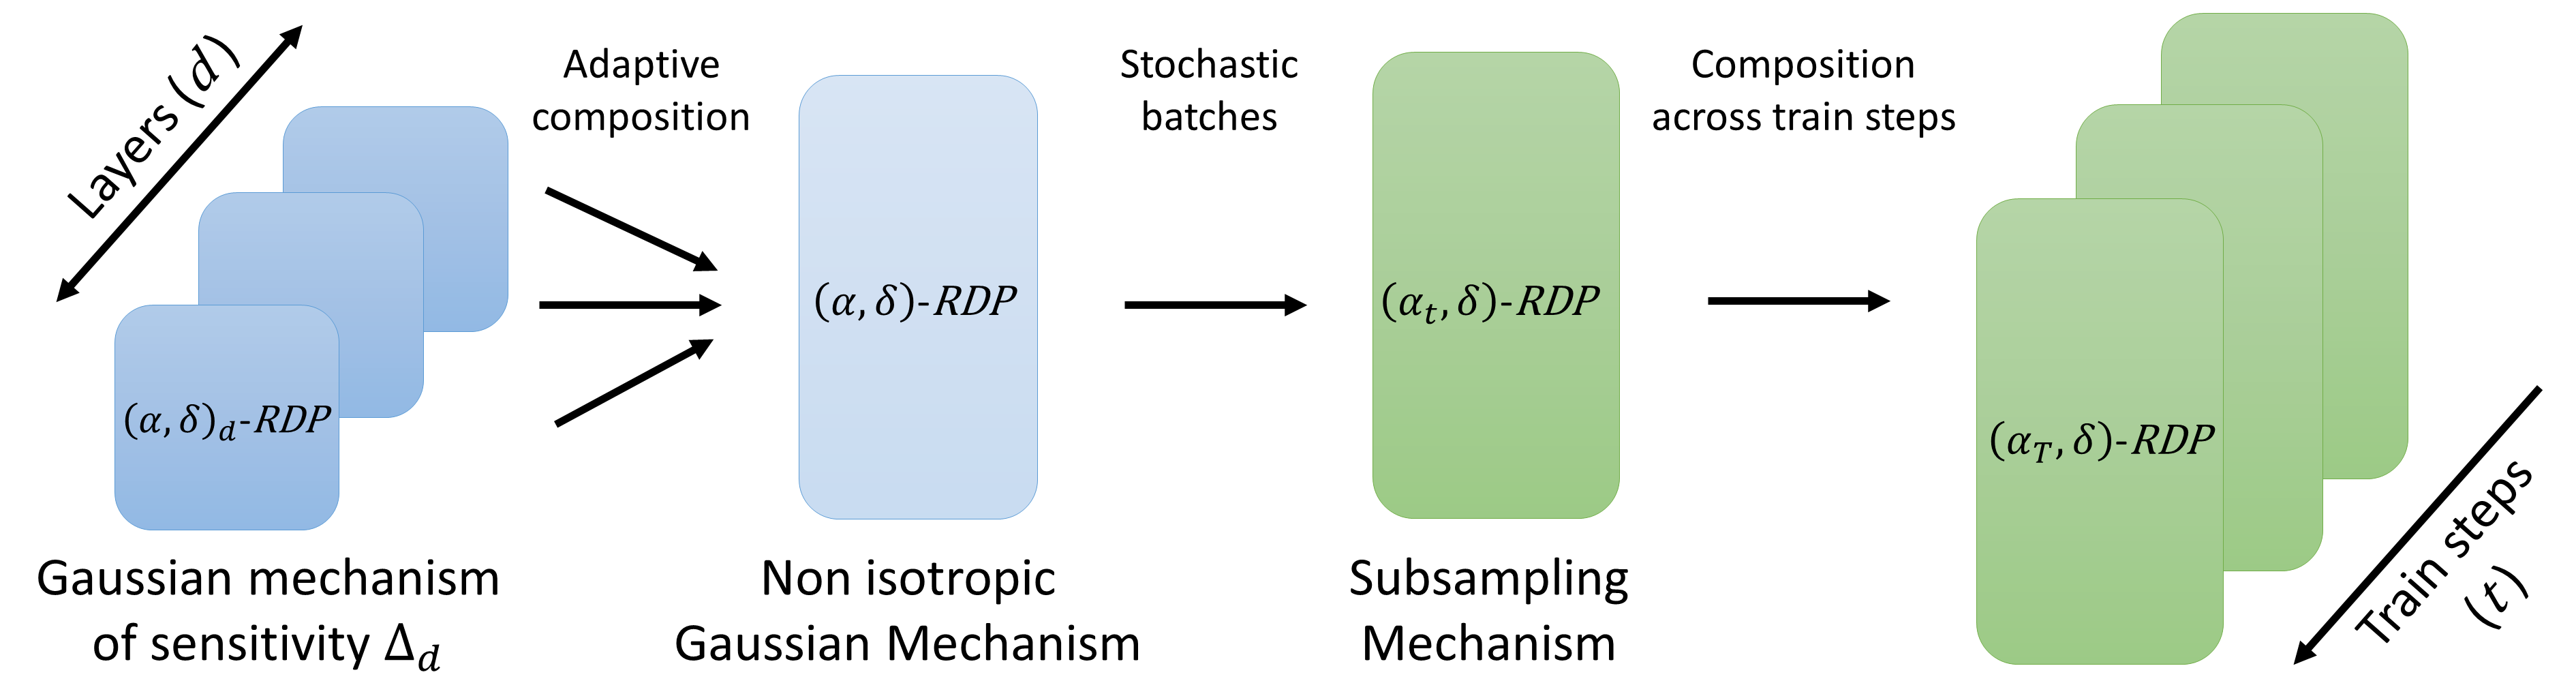
\includegraphics[width=\linewidth]{figures/fig_accountant.png}
        \caption{\textbf{Accountant for locally enforced differential privacy.} \textbf{(i)} The gradient query for each layer is made private using the Gaussian mechanism~\cite{dwork2014algorithmic}; \textbf{(ii)} their composition across the layers of the whole network can be seen as a non isotropic Gaussian mechanism, \textbf{(iii)} that benefits from amplification via sub-sampling~\cite{balle2018privacy}; \textbf{(iv)} the train steps are composed over the course of training.}
        \label{fig:local_accounting}
    \end{figure}    

\subsection{Privacy accounting of Clipless DP-SGD} \label{sec:cliplessSGD}

    \textbf{The ``global'' strategy.}
    This strategy simply aggregates the individual sensitivities $\sntv_d$ of each layer to obtain the global sensitivity of the whole gradient vector $\Delta=\sqrt{\sum_{d} \Delta_d^2}$. The origin of the clipping-based version of this strategy can be traced back to~\cite{mcmahanlearning}. With noise variance $\sigma^2\sntv^2$ we recover the accountant that comes with DP-SGD. It tends to overestimate the true sensitivity (in particular for deep networks), but its implementation is straightforward with existing tools. We detail in Algorithm~\ref{alg:noclipdpsgd} the global variant of our approach. 

    \paragraph{The ``per-layer'' strategy.} Recall that we are able to characterize the sensitivity $\Delta_d$ of every layer of the network. Hence, we can apply a different noise to each of the gradients. We dissect the whole training procedure in Figure~\ref{fig:local_accounting}.   
    \begin{enumerate}
        \item On each layer, we apply a Gaussian mechanism with noise variance $\sigma^2\Delta_d^2$. %The accountant only requires the noise multiplier $\sigma_d$.
        \item Their composition yields an other Gaussian mechanism with non isotropic noise.
        \item The Gaussian mechanism benefits from privacy amplification via subsampling~\citep{balle2018privacy} thanks to the stochasticity in the selection of batches of size $b=pN$.
        \item Finally an epoch is defined as the composition of $T=\frac{1}{p}$ sub-sampled mechanisms.
    \end{enumerate}
     At same noise multiplier $\sigma$, ``per-layer'' strategy tends to produce a higher value of $\epsilon$ per epoch than the ``global'' strategy, but has the advantage over the latter to add smaller effective noise $\zeta$ to each weight.  Different layers exhibit different maximum gradient bounds - and in turn this implies different sensitivities. This also suggests that different noise multipliers $\sigma_d$ can be used for each layer. This open extensions for future work.  

    For practical computations, we rely on the \lstinline[basicstyle=\ttfamily, backgroundcolor=\color{gray!20}]{autodp} library~\citep{wang2019subsampled,zhu2019poission,zhu2020improving} as it uses the R\'enyi Differential Privacy (RDP) adaptive composition theorem~\citep{mironov2017renyi,mironov2019r}, that ensures tighter bounds than naive DP composition.

    \begin{algorithm}%[tb]
    \caption{\textbf{Clipless DP-SGD} with \textbf{global} sensitivity accounting}
    \label{alg:noclipdpsgd}
    \textbf{Input}: Feed-forward architecture $f(\cdot,\cdot)=f_{T+1}(\theta_{T+1},\cdot)\circ f_T(\theta_T,\cdot)\circ \ldots \circ f_0(\theta_0,\cdot)$\\
    \textbf{Input}: Initial weights $\theta_0$, learning rate scheduling $\eta_t$, noise multiplier $\sigma$.%\\
    \begin{algorithmic}[1] %[1] enables line numbers.
    \Repeat
        \State $\Delta_0\ldots \Delta_{T+1}\gets $ compute\_gradient\_bounds$(f, X).$
        \State Sample a batch $\mathcal{B}_t=\{(x_1, y_1), (x_2, y_2), \ldots, (x_b, y_b)\}$.
        \State Compute the mean gradient of the batch for each layer $t$: 
            $$\tilde g_{t}\defeq \frac{1}{b} \sum_{i=1}^b \nabla_{\theta_{t}} \Loss (\yhat_i,y_i)).$$
        \State For each layer $t$ of the model, get the theoretical bound of the gradient: $$\forall 1 \leq i \leq b,\quad \|\nabla_{\theta_t} \Loss (\yhat_i,y_i)\|_2 \leq \Delta_t.$$
        \State Update Moment accountant state with \textbf{global} sensitivity $\Delta=\frac{2}{b}\sqrt{\sum_{t=1}^{T+1} \Delta_t^2}$.  
        \State Add global noise $\zeta \sim \mathcal{N}(0,2\sigma \Delta/b)$ to each weights and perform projected gradient step:
            $$\theta_{t}\gets \Pi(\theta_{t}-\eta (\tilde g_{t} + \zeta)).$$
        \State Report new $(\epsilon,\delta)$-DP guarantees with accountant.
    \Until{privacy budget $(\epsilon,\delta)$ has been reached.}
    \end{algorithmic}
    \end{algorithm}

\subsection{Robustness certificates of Lipschitz constrained networks}  

    The temperature parameter $\tau$ of softmax has a strong influence on the certificates. The models with the most robust decisions are not the ones with the best clean accuracy, which is compliant with the observations of~\cite{bethune2022pay}.  
    
    \begin{table*}
    \centering
    \small
    \begin{tabular}{|c|cccccc|cc|}
    \hline
      \multirow{3}{4.5em}{\centering Softmax Temperature} & \multicolumn{6}{c|}{\multirow{2}{*}{Certifiable accuracy at radius $r/255$}} &  \multicolumn{2}{c|}{\multirow{2}{7em}{\centering Membership Inference Attacks}}\\
        &       &       &       &       &       &               &       &     \\
        & $r=0$ & $r=1$ & $r=2$ & $r=4$ & $r=8$ & $r=16$        & AUROC & Adv.\\ 
    \hline
    \hline
    $\tau=0.01$ & $\bm{47.4}$ & $5.9$ & $0.1$ & $0.0$ & $0.0$ & $0.0$ & $59.8$ & $23.9$\\
    $\tau=0.22$ & $44.4$ & $\bm{39.1}$ & $34.2$ & $24.9$ & $11.5$ & $0.8$ & $50.1$ & $15.0$\\
    $\tau=0.40$ & $41.6$ & $38.4$ & $\bm{35.6}$ & $29.6$ & $19.1$ & $5.3$ & $50.0$ & $11.3$\\
    $\tau=0.74$ & $38.4$ & $36.4$ & $34.7$ & $\bm{30.9}$ & $24.1$ & $13.0$ & 51.9 & 20.5\\
    $\tau=2.77$ & $33.3$ & $32.2$ & $31.2$ & $29.3$ & $\bm{25.9}$ & $18.8$ & 52.5 & 21.3\\
    $\tau=5.40$ & $32.5$ & $31.4$ & $30.4$ & $28.8$ & $25.5$ & $\bm{19.7}$ & 59.7 & 23.6\\
    \hline
    \end{tabular}
    \caption{\textbf{Certifiable accuracy scores under ($20.0$, $10^{-5}$)-DP training on Cifar-10 dataset}. For each targeted robustness radius $r/255$, we optimize over softmax-crossentropy temperature $\tau$, and report the best value. We also monitor the best AUROC and the best attacker Advantage (Adv.)~\cite{yeom2018privacy} achieved by two popular membership inference attacks: threshold attacks~\cite{song2021systematic} and a logistic regression shadow model~\cite{shokri2017membership}.}
    \label{tab:certificates}
    \end{table*}

\rebuttal{    
\subsection{Bias of Clipless DP-SGD}\label{sec:discussionbias}

    Clipless DP-SGD \textit{also} exhibits a bias, but this bias takes a different form than the bias induced by clipping in DP-SGD.

    \paragraph{The bias of the optimizer.} In DP-SGD (with clipping) the average gradient is biased by the elementwise clipping. Therefore, the clipping may slow down convergence or lead to sub-optimal solutions.  

    \paragraph{The bias of the model in the space in Lipschitz networks.} This is a bias of the model, not of the optimizer. It has been shown that any classification task could be solved with a 1-Lipschitz classifier~\citep{bethune2022pay}, and in this sense, the bias induced by the space of 1-Lipschitz functions is not too severe. Better, this bias is precisely what allows to produce robustness certificates, see for example~\cite{yang2020closer}.  
    
    \paragraph{Finally, there is the implicit bias.} It is induced by a given architecture on the optimizer, which can have strong effects on effective generalization. For neural networks (Lipschitz or not), this implicit bias is not fully understood yet. But even on large Lipschitz models, it seems that the Lipschitz constraint biases the network toward better robustness radii but worse clean accuracy, as frequently observed in the relevant literature.
    
    Therefore, these biases influence the learning process differently, and they constitute two distinct (not necessarily exclusive) approaches. We illustrate the difference between these paradigms in Figure~\ref{fig:allthebiases}.  

\subsection{Efficiency of gradient clipping}\label{sec:comparisonsota}

    Beyond the conventional implementation of gradient clipping that can be found in Opacus or Tf-privacy, recent developments proposed more efficient forms of clipping, or to get rid of the clipping introduced by~\cite{abadi2016deep} and to use renormalization instead.  
      
    In this regard, we can mention the works of~\cite{bu2022automatic} or~\cite{yang2022normalized} that study alternative implementations of clipping based on renormalization, which eliminates the need to tune the clipping value, with convergence guarantees.  

    Other works study the alternative implementation of elementwise clipping to reduce the computational cost, like~\cite{bu2022scalable}, \cite{li2021large} \cite{he2022exploring}, and \cite{bu2023differentially}. Taking inspiration from~\cite{bu2023differentially} we summarize each one in Tables~\ref{tab:comparisonsota} and ~\ref{tab:comparisoncomplexity}.  

    \begin{table}[]
    \small
    \hspace{-1.4cm}
    %\centering
    \begin{tabular}{|c|ccccc|}
            \hline
        & \makecell{Instantiating\\ per-sample\\ gradient} & \makecell{Storing every\\ layer's gradient} & \makecell{Instantiating\\ non-DP\\ gradient} & \makecell{Number of\\ back-propagations} & \makecell{Overhead\\ independent of\\ batch size}\\
        \hline
        \hline
        non-DP & \cross & \cross & \checkmark & 1 & \checkmark \\
        TF-Privacy, like~\cite{abadi2016deep} & \checkmark & \cross & \checkmark & B & \cross \\
        Opacus~\citep{opacus} & \checkmark & \checkmark & \checkmark & 1 & \cross \\
        FastGradClip~\citep{lee2021scaling} & \checkmark & \cross & \cross & 2 & \cross \\
        GhostClip~\citep{li2021large,bu2022scalable} & \cross & \cross & \checkmark & 1 & \cross \\
        Book-Keeping~\citep{bu2023differentially} & \cross & \cross & \cross & 1 & \cross \\
        Clipless w/ Lipschitz (ours) & \cross & \cross & \checkmark & 1 & \checkmark\\
        Clipless w/ GNP (ours) & \cross & \cross & \checkmark & 1 & \checkmark\\
        \hline
        \end{tabular}
    \caption{\rebuttal{\textbf{Comparison of DP-SGD against existing techniques of literature}. Clipless DP-SGD is the only technique whose time/memory overhead depends exclusively on weight matrices but not the batch size.}}
    \label{tab:comparisonsota}
\end{table}

    \begin{table}
        \centering
        \begin{tabular}{|c|cc|}
        \hline
        & Time Complexity Overhead & Memory Overhead \\
        \hline
        \hline
        non-DP & 0 & 0 \\
        TF-Privacy, like~\cite{abadi2016deep} & $\BigO(BTpd)$ & 0 \\
        Opacus~\citep{opacus} & $\BigO(BTpd)$ & $\BigO(Bpd)$ \\
        FastGradClip~\citep{lee2021scaling} & $\BigO(BTpd)$ & $\BigO(Bpd)$ \\
        GhostClip~\citep{li2021large,bu2022scalable} & $\BigO(BTpd+BT^2)$ & $\BigO(BT^2)$ \\
        Book-Keeping~\citep{bu2023differentially} & $\BigO(BTpd)$ & $\BigO(B\min(pd, T^2))$ \\
        Clipless w/ Lipschitz (ours) & $\BigO(Upd)$ & 0\\
        Clipless w/ GNP (ours) & $\BigO(Upd+Vpd\min(p,d))$ & 0\\
        \hline
        \end{tabular}
        \caption{\rebuttal{\textbf{Time and memory costs for each method} for feedforward networks. We assume weight matrices of shape $p\times d$, and a \textit{physical} batch size $B$. For images, $T$ is height$\times$width. $U$ is the number of iterations in Power Iteration algorithm, and $V$ the number of iterations in Bj\"orck projection. Typically $U,V<15$ in practice. The overhead is taken relatively to non-DP training \textit{without} clipping. This table is largely inspired from~\cite{bu2023differentially}.}}
        \label{tab:comparisoncomplexity}
    \end{table}
}


\begin{figure}
    \centering
    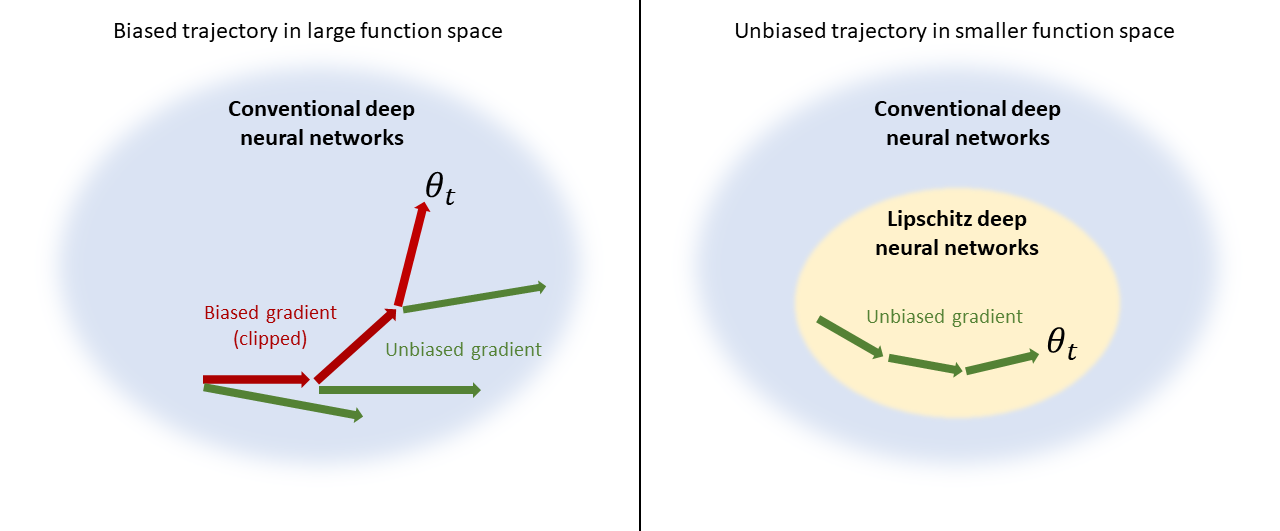
\includegraphics[width=1\linewidth]{figures/biasedfunctions.png}
    \caption{\rebuttal{Comparison between the bias of DP-SGD \textit{with} clipping, and Clipless DP-SGD. One is an instance of \textit{optimizer bias}, and the other of \textit{function space bias}.}}
    \label{fig:allthebiases}
\end{figure}
